\documentclass{article}
\usepackage{graphicx}
\usepackage{tocloft} 
\usepackage{glossaries}
\usepackage{lipsum}
\usepackage{geometry}
\usepackage{fancyhdr} 
\usepackage{amsmath}
\usepackage{biblatex}  

\addbibresource{../common/references.bib}  

\geometry{a4paper, margin= 1in}

\makeglossaries
\loadglsentries{../common/glossary.tex}

\title{Software Design Document (SDD)}
\author{Group 1 }
\date{December 3 2024}

\begin{document}
\maketitle  
\pagebreak

\tableofcontents
\pagebreak

\section*{Version History}
\begin{longtable}{|c|c|p{10cm}|}
\hline
\textbf{Version} & \textbf{Date} & \textbf{Description} \\ \hline
5.0 & December 3 2024 & Made Adjustments \\ \hline
4.0 & December 3 2024 & Finished document \\ \hline
3.0 & December 1 2024 & Finished Section 2.1 \\ \hline
2.0 &November 20, 2024 & Added glossary and references \\ \hline
1.0 & November 20 2024 & Began document and laid out the foundation \\ \hline
\end{longtable}
\pagebreak


\includegraphics[width=0.3\linewidth]{../logo/csula.png} 

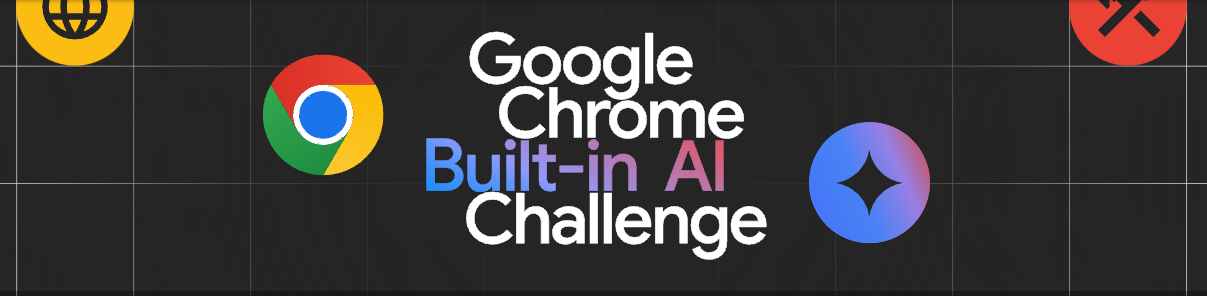
\includegraphics[width=0.3\linewidth]{../logo/chromeai.png} 

\section{Introduction}

\subsection{Purpose}
Our project is based on a competition from Google to use Chrome's built-in \Gls{ai} APIs to interact with Gemini Nano or other AI models in a web app or Chrome browser extension. 

The competition is available at \url{https://googlechromeai.devpost.com/}

\subsection{Intended Audience}
Our Project Management System is designed to cater to Project Managers, Software Teams, Technical Stakeholders, and any individual or organization that requires a project management tool and values AI integration for task management. Whether it's automating task descriptions, simplifying project oversight, or improving team collaboration, our system is designed to meet the needs of both small teams and large organizations looking to optimize their project management processes.

\subsection{Overview}
Our web application is a Project Management System similar to TestRails or Jira. Using the built-in Chrome \Gls{ai} API, we will include AI-generated descriptions and task creations with voice input. We use the Chrome developer documentation\cite{dev} as the main reference for developing a Chrome extension.

\section{System Architecture}

\subsection{Workflow}

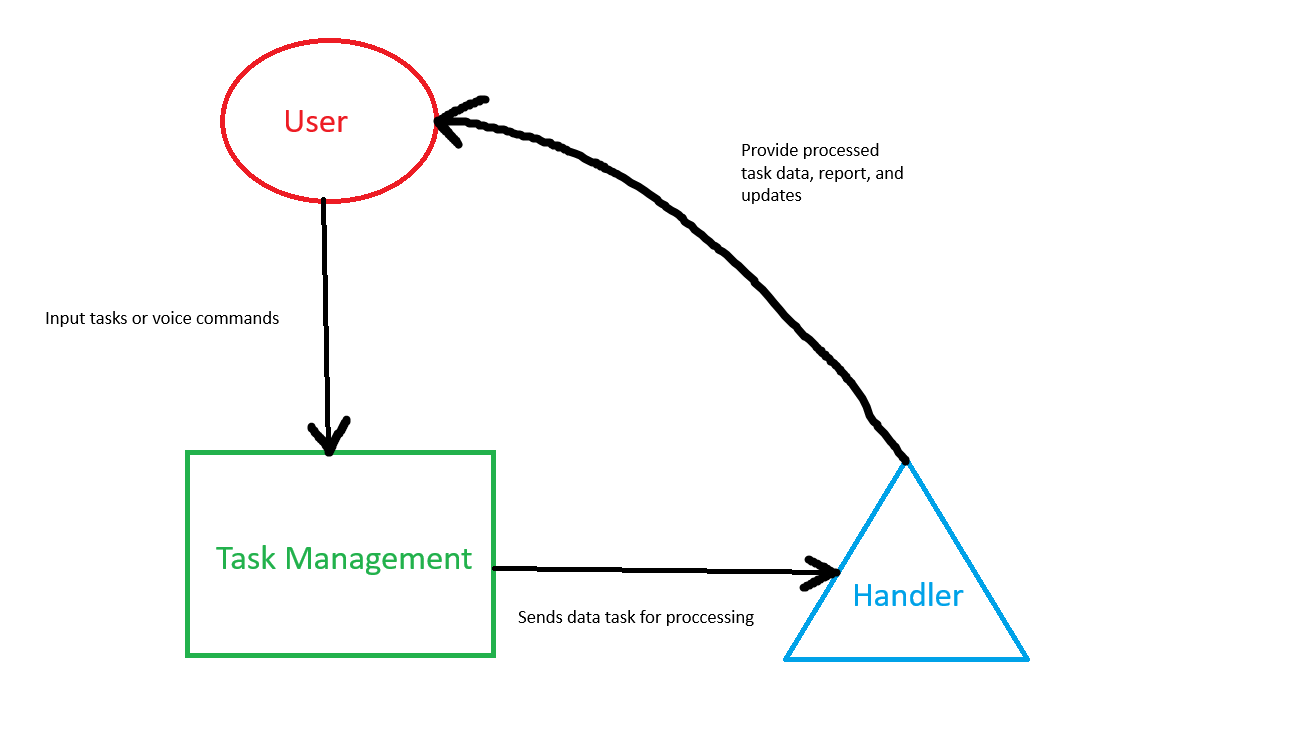
\includegraphics[width=0.9\linewidth]{../logo/workflow.png} 

\begin{itemize}
    \item User: The user interacts with the system through the Chrome extension interface. Voice inputs are then captured using the user's microphone for task creation. Commands and inputs are sent to the server for processing.
    \item AI-Driven Task Management: User inputs are analyzed by AI algorithms on the server. AI generates task descriptions and suggestions, which are then sent back to the client-side for user review.
    \item Data Handler: Task and project data are stored and retrieved from a central database. Real-time updates are sent to clients.
    \item Project Update: Updates are processed and visualized on the dashboard in real time. AI-generated insights are displayed to the user.
\end{itemize}

\section{User Interface}

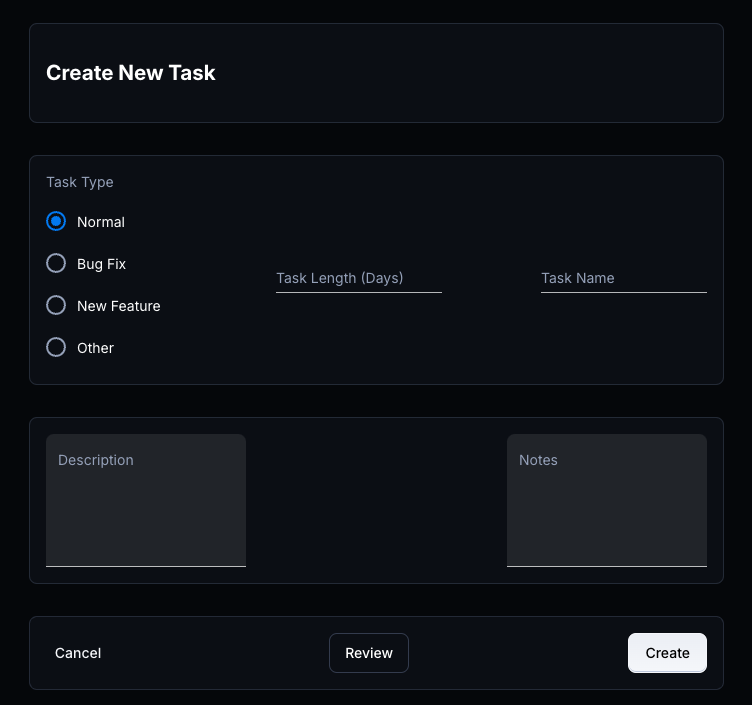
\includegraphics[width=0.9\linewidth]{../logo/mockup.png} 

The UI is based on Material UI\cite{mui}. The create-new-task page is shown above. It includes various options such as specifying the type of task you wish to create, choosing a duration for the task, and adding any additional notes the user may wish to include.

\subsection{UI Features and Accessibility}
The user interface is designed to ensure a smooth and intuitive user experience, with the following key considerations:
\begin{itemize}
    \item **Material UI Framework:** Ensures consistent, professional design with responsive elements that adapt to different screen sizes.
    \item **Accessibility Features:**
    \begin{itemize}
        \item High-contrast mode for improved readability.
        \item Keyboard navigation for users who prefer or require non-mouse input methods.
        \item Screen reader support for visually impaired users.
    \end{itemize}
    \item **Responsiveness:** The layout adapts seamlessly to mobile, tablet, and desktop devices.
    \item **User-Friendly Navigation:** Key actions, such as creating tasks or viewing project dashboards, are accessible through intuitive buttons and dropdown menus.
\end{itemize}

\subsection{Database Design}
The database is a straightforward \Gls{sql} layout with a UserID lookup table and a main task table. Users can only access tasks that were created by or shared with their UserID. The UserID lookup table associates each user with a unique ID, ensuring secure and efficient access to user-specific data.

\begin{itemize}
    \item **UserID Lookup Table:**
    \begin{itemize}
        \item Contains a unique identifier for each user.
        \item Links user accounts to their respective tasks.
    \end{itemize}
    \item **Main Task Table:**
    \begin{itemize}
        \item Stores details about tasks, including:
        \begin{itemize}
            \item Task descriptions.
            \item Deadlines.
            \item Statuses (e.g., pending, completed).
        \end{itemize}
        \item Enforces access control, ensuring users can view or modify only their tasks or tasks explicitly shared with them.
    \end{itemize}
\end{itemize}

This database structure ensures data integrity, privacy, and seamless task management across the platform.

\pagebreak
\section{Glossary}
\printglossaries

\pagebreak
\section{References}
\printbibliography
\end{document}